% !TEX root = ../../../Masterthesis.tex
\section{Attack Pattern}\label{sec:attack pattern}
%-----------------------------------------------------------------------------
% Part ABC
%-----------------------------------------------------------------------------
\begin{figure}[h!]
\center
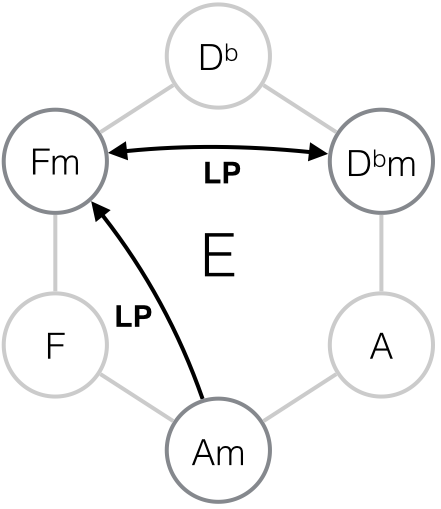
\includegraphics[width=0.5\linewidth]{ST10_attack_pattern_abce}
	\caption{ST 10: Attack Pattern, part A, B, C and E}
	\label{ST10_attack_pattern_abce}
	\setfloatalignment{b}
\end{figure}
\noindent Captain Picard and Lt. Cdr. Data are conversing in the cartography room when they realize they are going to lose long range communications. The music starts at the moment of realization. It is a tension-building, syncopated motif in \lilyTimeSignature{7}{4} played by the low strings (figure \ref{ST10_attack_pattern_abce}). A sweeping synth and horns play the second motif as both Data and Picard realize that this is the moment Shinzon has been waiting for. Picard orders evasive maneuvers, but Shinzon has already begun the attack. The tonality is exclusively octatonic\marginnote{\keyboard{C,Ciss,Diss,E,Fiss,G,A,Aiss}}, giving the overall sonority, combined with odd meters, an aggressive and uneasy nature. Enterprise is critically hit and loosing warp capabilities. Shinzon's ship is seen turning around to continue the attack. The musical meters adapt to mickey-mouse the cuts. 

The music drops in energy and a new motif enters, \textbf{C}, as we cut to the interior of Shinzon's ship where the attack on the Enterprise continues. Picard returns to the bridge and orders retaliation and the music picks up again. Shinzon's ship is cloaked and, ultimately, the Enterprise manages to inflict only minimal damage. 

The music, now at letter \textbf{C}, introduces a new motif, \textit{motif 3} accompanied by \textit{motif 1}. All in all, it is very subdued and clearly restrained, mirroring the screen as there is a momentary absence of fire. The crew of Enterprise gives rapports on current status. 

\begin{marginfigure}
%\center
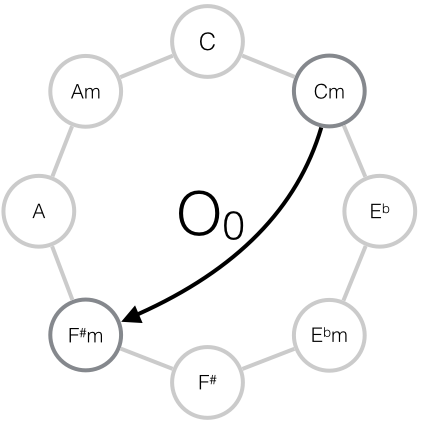
\includegraphics[width=\linewidth]{ST10_attack_pattern_D}
	\caption{ST 10: Attack Pattern, part D and E}
	\label{ST10_attack_pattern_D}
	%\setfloatalignment{b}
\end{marginfigure}

Shinzon plans his ferocious attack, and Goldsmith does the first, and only network modulation, to Cm (figure \ref{ST10_attack_pattern_D}). From letter \textbf{E} the planning evolves, and letter \textbf{F} is introduced simultaneously as the attack explodes into action. The battle ends when the Enterprise can take no more; Shinzon hails Picard and the battle ends. 
%-----------------------------------------------------------------------------
% PDF
%-----------------------------------------------------------------------------
\clearpage
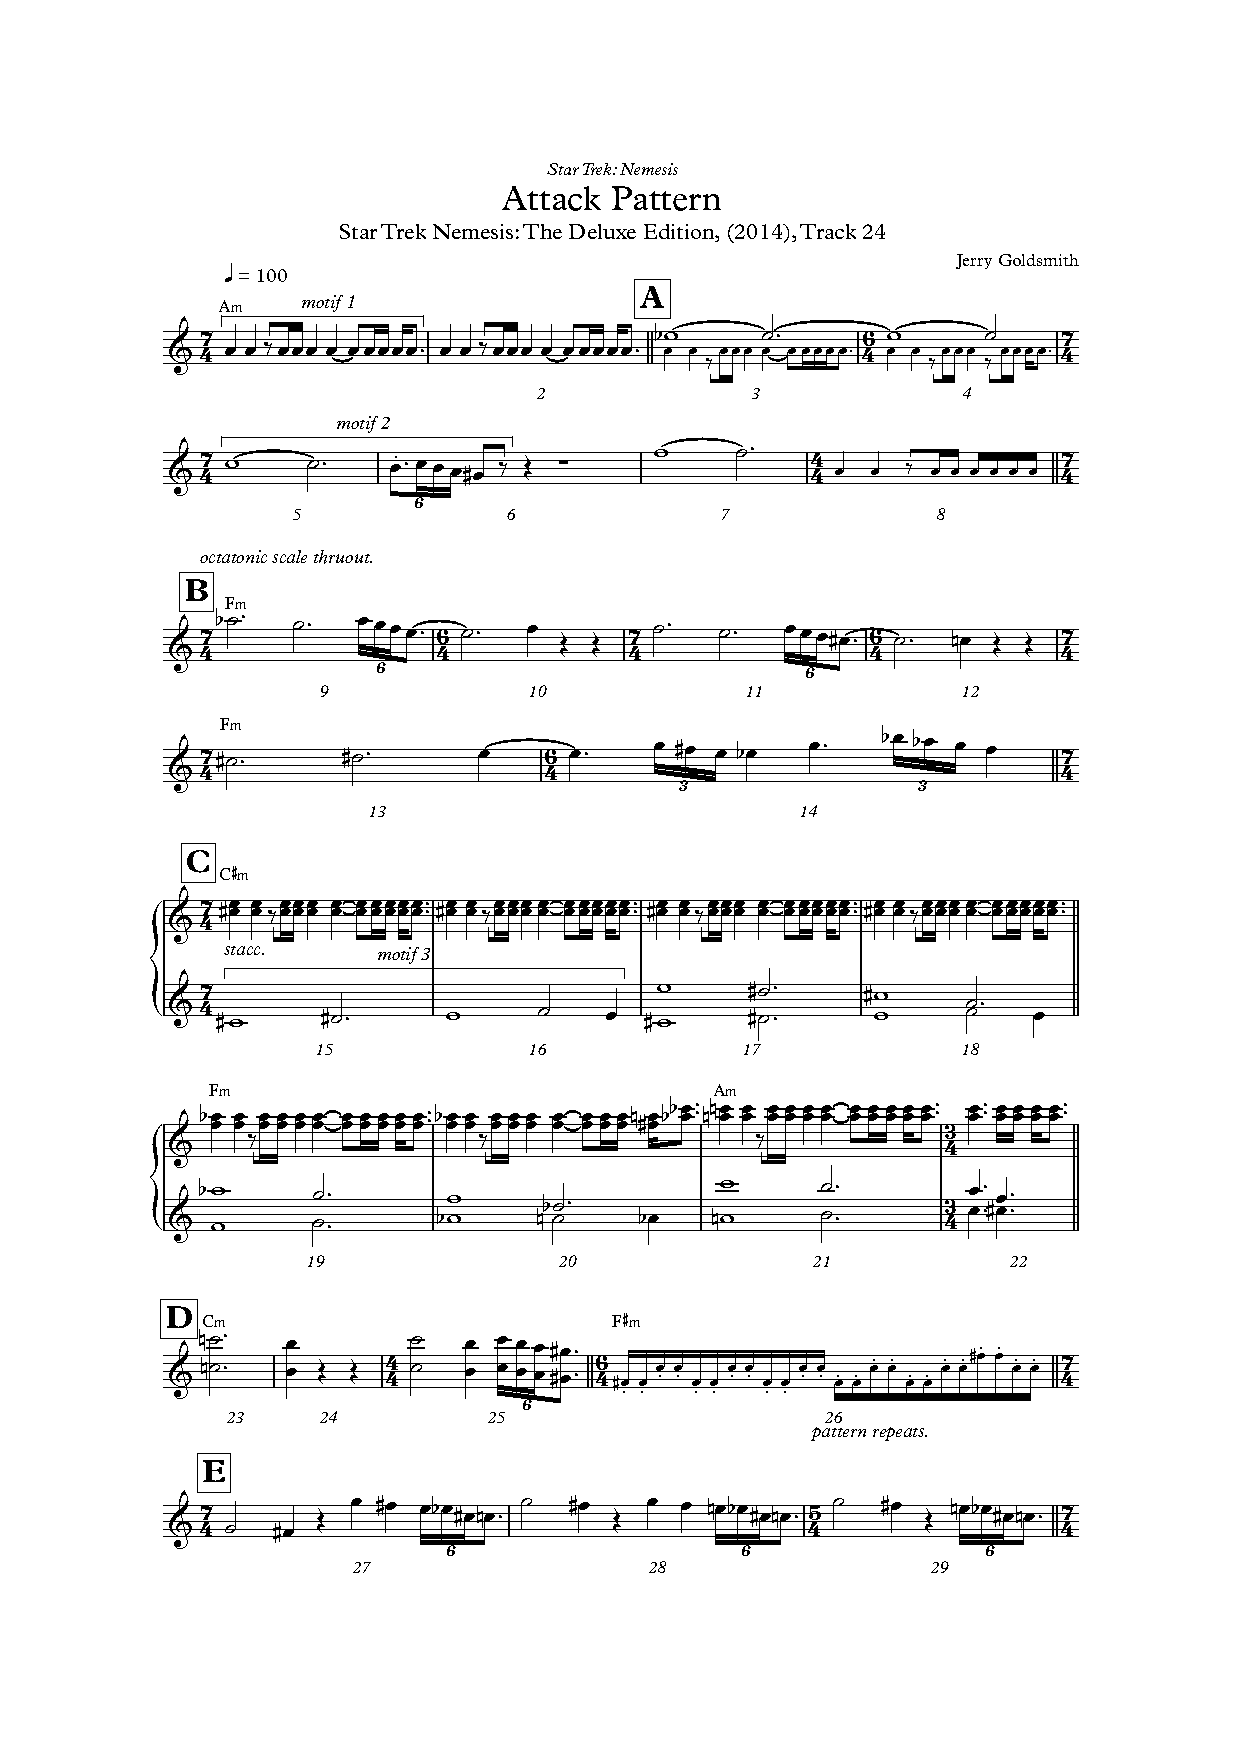
\includepdf[pages=-,pagecommand=\thispagestyle{fancy}]{pdf/st10/ST10_Attack_Pattern} 

% Reviewed